\documentclass[11pt]{article}

% set these commands
\newcommand{\course}{CSCI 534}
\newcommand{\proj}{Homework 04}
\newcommand{\dueDate}{3-18-2019}
\newcommand{\instructor}{David L. Millman}

\usepackage{macros}

\begin{document}

{ ~\\
    \course \\ 
    \proj \\ 
    Due \dueDate \\
    \instructor
}

\section*{Problem 1 (5 points)}

Draw a polygon with at least 4 vertices and give each vertex coordinates.
Using the duality discussed in class, draw the dual of the polygon.  In the
dual,
\begin{itemize}
    \item shade black the duals of the points that are on the vertices in the primal
    \item shade grey the duals of the points that are on the edges in the primal
    \item shade red the duals of the points that are inside the polygon in the primal
\end{itemize}

You should draw the primal and dual to scale.  You may draw the figure by hand,
but, I suggest using a tool like Ipe or Inkscape.

\section*{Problem 2 (20 points)}

Explain how to solve each of the following problems in linear (expected) time.
Each can be modeled as a linear programming (LP) problem, perhaps with some
additional pre- and/or post- processing. In each case, explain how the problem
is converted into an LP instance and how the answer to the LP instance is
used/interpreted to solve the stated problem.

\begin{enumerate}

    \item You are given two point sets $P = \{p_1,\ldots,p_n\}$ and $Q =
        \{q_1,\ldots,q_m\}$ in the plane, and you are told that they are
        separated by a vertical line $x = x_0$, with $P$ to the left and $Q$ to
        the right (see Fig. a). Compute the line equations of the two
        ``crossing tangents,'' that is, the lines $\ell_1$ and $\ell_2$ that are
        both supporting lines for $\rm{conv}(P)$ and $\rm{conv}(Q)$ such that
        $P$ lies below $\ell_1$ and above $\ell_2$ and the reverse holds for
        $Q$. (Note that you are not given the hulls, just the point sets.) Your
        algorithm should run in time $O(n + m)$.

    \begin{figure}[h]
        \centering
        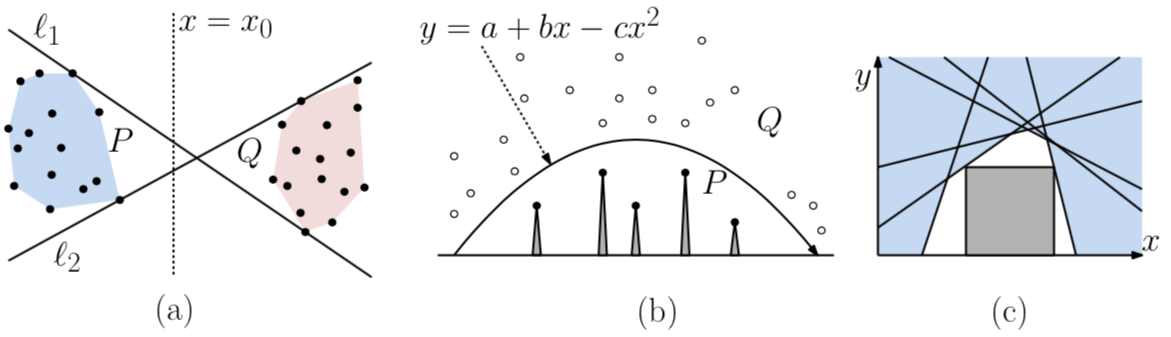
\includegraphics[width=0.75\textwidth]{lp}
        \caption{Problem 3: LP applications}
    \end{figure}


    \item You have a cannon in $\R^2$. It has three controls labeled ``a'' ``b,''
        and ``c''. A projectile shot from this cannon travels along the
        parabolic arc $y = a + bx - cx^2$. You are asked to determine whether it
        is possible to adjust the controls so that the projectile travels above
        a set of $n$ building tops, represented by a point set $P = \{p_1,
        \ldots , p_n\}$ and beneath a set of $m$ floating balloons, represented
        by a point set $Q = \{q_1, \ldots , q_m\}$ (see Fig. b)). Your algorithm
        should run in time $O(n + m)$. (I do not care where the cannon is
        actually located. If your solution is based on some assumption about the
        cannon's location, please state this.)

    \item You are given a set of $n$ halfplanes $H = \{h_1,\ldots,h_n\}$, where
        $h_i$ is given as a pair $(a_i,b_i)$ and it consists of all the points
        of the plane that lie on or beneath the line $y = a_ix + b_i$. Compute
        the axis-parallel square of the largest side length whose lower edge
        lies on the x-axis (see Fig.~c). If no such square exists, your
        algorithm should indicate this.

\end{enumerate}

\section*{Tips and Acknowledgements}

{\bf Acknowledgements:} Homework problems adapted from assignments of David
Mount and Carola Wenk.

\end{document}
